% Results -- figures and tables: Kaiyuan Xu; analysis: everyone (draft, edit freely).
% % Results -- figures and tables: Kaiyuan Xu; analysis: everyone (draft, edit freely).
% % Results -- figures and tables: Kaiyuan Xu; analysis: everyone (draft, edit freely).
% % Results -- figures and tables: Kaiyuan Xu; analysis: everyone (draft, edit freely).
% \input{results} from the main report. Every number below comes from
% results/summary/final.md (python experiments/final_figures.py); the table and
% figures are generated files, so rerun that script rather than editing them.
% TODO(Sicheng): \label{sec:sensitivity} and \label{sec:lanes} are referenced
% below for the matched-window and lane studies; adjust if your labels differ.

\section{Results}
\label{sec:results}

All 2{,}040 test runs completed every task with no conflicts. Table~\ref{tab:main}
gives the mean paired change of each method against TP over the 90 pairs per
map (10, 30 and 50 agents; 0.2, 1 and 5 tasks per step; seeds 0--9).
Under TP the mean service time is 122.6 timesteps on \texttt{warehouse\_small}
and 184.3 on \texttt{narrow\_corridor}, with 0.49 and 0.82 head-on encounters
per task.

\begin{table}[t]
  \centering\small
  \caption{Mean paired change vs.\ TP (\%), 90 pairs per map
  (W = \texttt{warehouse\_small}, N = \texttt{narrow\_corridor}). $^*$: Wilcoxon
  signed-rank $p<0.05$. Lower is better in every column.}
  \label{tab:main}
  \input{../results/summary/final_table}
\end{table}

\paragraph{Every congestion cost removes about half of the head-on encounters.}
Every path cost lowers head-on encounters in all 90 of 90 pairs on both maps
(Fig.~\ref{fig:headon}): by 39--53\% on \texttt{warehouse\_small} and by
50--54\% on \texttt{narrow\_corridor}, except M3 there ($-15.5\%$). The tuned
time-resolved costs M4 and M5 are among the largest reductions on both maps.

\begin{figure}[t]
  \centering
  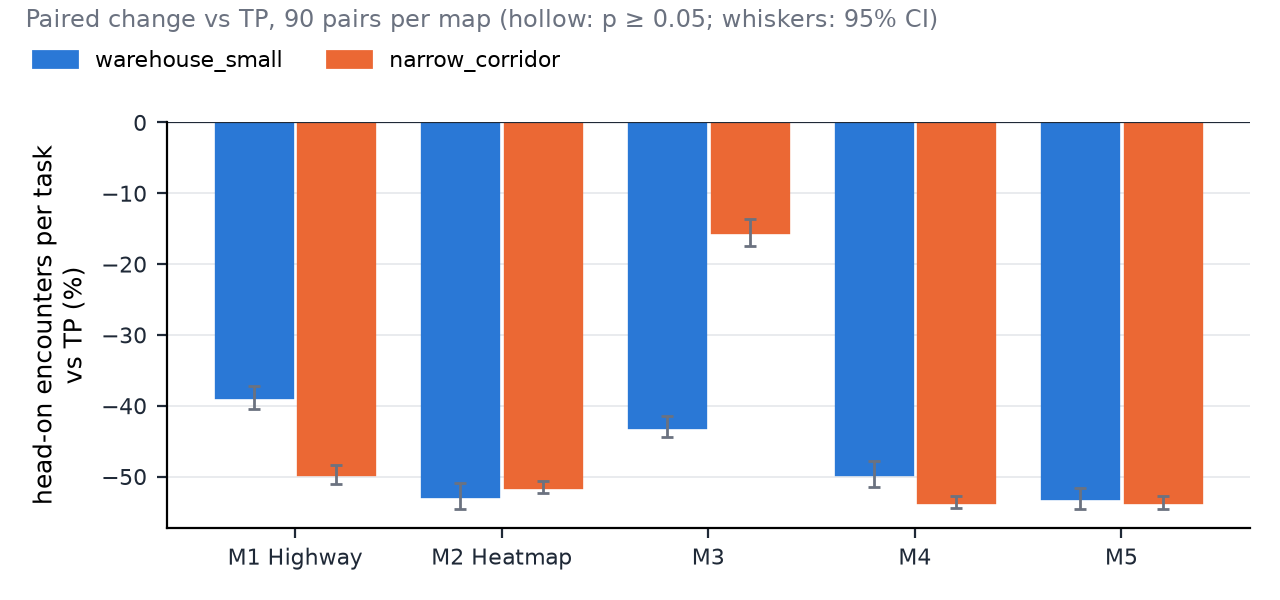
\includegraphics[width=\linewidth]{../results/summary/final_head_on.png}
  \caption{Head-on encounters per task, paired change vs.\ TP.}
  \label{fig:headon}
\end{figure}

\paragraph{Fewer encounters do not mean faster delivery; robots wait instead.}
Path costs change the mean service time by at most 2\%. On
\texttt{warehouse\_small} M2--M5 are slightly but significantly faster than TP
($-0.9\%$ to $-1.9\%$) and also lower the 95th percentile ($-0.5\%$ to
$-1.5\%$); on \texttt{narrow\_corridor} none of them differs significantly from
TP, and Highway is no faster on \texttt{warehouse\_small} and slower on
\texttt{narrow\_corridor} ($+1.1\%$). The wait fraction rises instead: by
13.5--57\% on \texttt{warehouse\_small} and by 101--145\% on
\texttt{narrow\_corridor} for every method except M3. Agents trade a head-on
encounter for waiting before an aisle, which leaves the service time almost
unchanged.

\paragraph{Contribution 1: timing matters for encounters, not for service time.}
With tuned parameters, M4 removes more encounters than M3 on both maps
($-49.7\%$ vs.\ $-43.0\%$ on \texttt{warehouse\_small}; $-53.6\%$ vs.\
$-15.5\%$ on \texttt{narrow\_corridor}). Tuning chose different window sizes
for M3 and M4 on \texttt{narrow\_corridor} (2 vs.\ $\delta=2$, i.e.\ 5 steps),
so the matched-window comparison in Section~\ref{sec:sensitivity} isolates the
effect of timing. The two do not differ in service time.

\paragraph{Contribution 2: no measurable effect of the direction term.}
M5 is within a few points of M4 on every metric (head-on $-53.1\%$ vs.\
$-49.7\%$ on \texttt{warehouse\_small}, $-53.7\%$ vs.\ $-53.6\%$ on
\texttt{narrow\_corridor}), consistent with the lane study
(Section~\ref{sec:lanes}), in which no one-way lanes form.

\paragraph{Looking forward does not beat looking backward.}
Compared directly with the tuned history heatmap M2 on the same pairs, M4 and
M5 are slightly slower on \texttt{warehouse\_small} ($+1.0\%$ and $+0.9\%$
mean service time, both significant) and indistinguishable on
\texttt{narrow\_corridor} ($+0.4\%$, not significant), where they have 4\%
fewer head-on encounters than M2 but wait 3\% more. Under heavier load (80
agents at 1 and 5 tasks per step, 20 pairs per map) M4 and M5 do lower the mean
and 95th-percentile service time on \texttt{narrow\_corridor} ($-2.5\%$ and
$-3.2\%$ for M4), but M2 does as well ($-3.0\%$ and $-3.4\%$). The forecast in
the token is exact, yet in these warehouses recent history predicts congestion
about as well.

\paragraph{Assignment helps more than routing.}
Choosing tasks with $S_{ij}$ instead of the nearest pickup lowers the mean
service time by 3.6\% on \texttt{warehouse\_small} and 1.5\% on
\texttt{narrow\_corridor} (both significant), more than any path cost
(Fig.~\ref{fig:ablation}). The gain adds to that of the path costs: M4~$+\,S_{ij}$
is 3.8\% and 1.3\% faster than TP, and adding $S_{ij}$ to M3, M4 or M5 lowers
the service time by a further 2.5--2.9\% and 1.0--1.3\%. $S_{ij}$ hardly
changes head-on encounters ($-2$\% to $-3.5\%$) and does not lengthen the
slowest tasks: on the test seeds the maximum service time is unchanged on
\texttt{warehouse\_small} ($+0.5\%$, not significant) and lower on
\texttt{narrow\_corridor} ($-1.6\%$). Routing and assignment therefore act on
different things: the path costs on encounters, the assignment on service
time.

\begin{figure}[t]
  \centering
  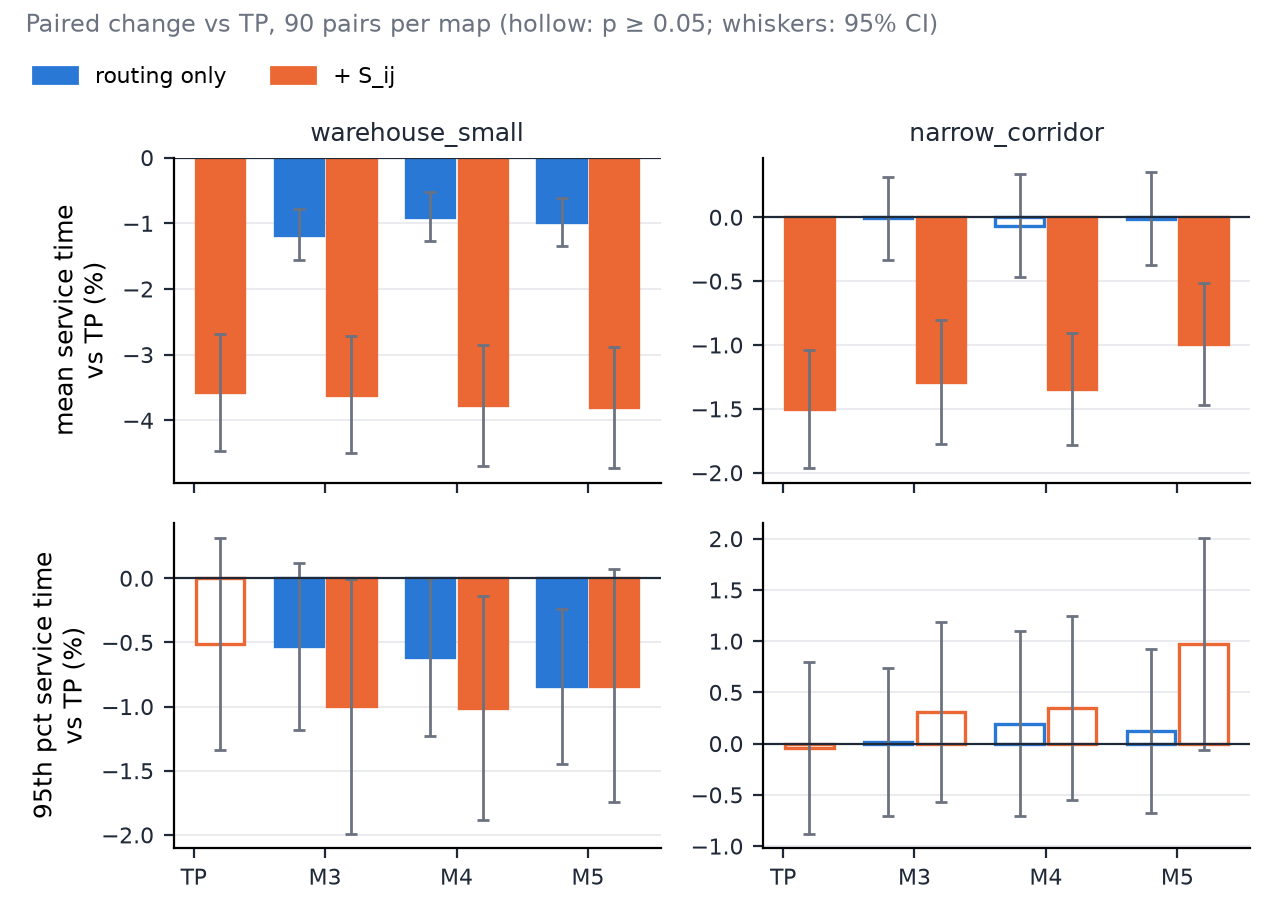
\includegraphics[width=\linewidth]{../results/summary/final_ablation.png}
  \caption{Routing vs.\ assignment: mean (top) and 95th-percentile (bottom)
  service time, paired change vs.\ TP.}
  \label{fig:ablation}
\end{figure}

\paragraph{Cost.}
Planning stays cheap. TP plans in about 0.65 ms per timestep on average on both
maps, and 1.9--2.6 ms at 80 agents. The congestion costs add 18--195\% depending on
method and map, and $S_{ij}$ adds up to 91\% on \texttt{warehouse\_small},
The slowest setting (M4, \texttt{narrow\_corridor}, 80 agents, 5 tasks per
step) averages 7.4 ms per timestep.
 from the main report. Every number below comes from
% results/summary/final.md (python experiments/final_figures.py); the table and
% figures are generated files, so rerun that script rather than editing them.
% TODO(Sicheng): \label{sec:sensitivity} and \label{sec:lanes} are referenced
% below for the matched-window and lane studies; adjust if your labels differ.

\section{Results}
\label{sec:results}

All 2{,}040 test runs completed every task with no conflicts. Table~\ref{tab:main}
gives the mean paired change of each method against TP over the 90 pairs per
map (10, 30 and 50 agents; 0.2, 1 and 5 tasks per step; seeds 0--9).
Under TP the mean service time is 122.6 timesteps on \texttt{warehouse\_small}
and 184.3 on \texttt{narrow\_corridor}, with 0.49 and 0.82 head-on encounters
per task.

\begin{table}[t]
  \centering\small
  \caption{Mean paired change vs.\ TP (\%), 90 pairs per map
  (W = \texttt{warehouse\_small}, N = \texttt{narrow\_corridor}). $^*$: Wilcoxon
  signed-rank $p<0.05$. Lower is better in every column.}
  \label{tab:main}
  % Generated by experiments/final_figures.py -- do not edit by hand.
\begin{tabular}{lrrrrrrrr}
\toprule
 & \multicolumn{2}{c}{Service time} & \multicolumn{2}{c}{p95 service} & \multicolumn{2}{c}{Head-on / task} & \multicolumn{2}{c}{Wait fraction} \\
 & W & N & W & N & W & N & W & N \\
\midrule
M1 Highway & +0.4 & +1.1$^*$ & +1.2 & +1.9$^*$ & $-$38.8$^*$ & $-$49.7$^*$ & +13.5$^*$ & +101.4$^*$ \\
M2 Heatmap & $-$1.9$^*$ & $-$0.4 & $-$1.5$^*$ & +0.1 & $-$52.8$^*$ & $-$51.5$^*$ & +22.1$^*$ & +137.8$^*$ \\
M3 & $-$1.2$^*$ & $-$0.0 & $-$0.5$^*$ & +0.0 & $-$43.0$^*$ & $-$15.5$^*$ & +17.3$^*$ & +40.8$^*$ \\
M4 & $-$0.9$^*$ & $-$0.1 & $-$0.6$^*$ & +0.2 & $-$49.7$^*$ & $-$53.6$^*$ & +56.7$^*$ & +144.8$^*$ \\
M5 & $-$1.0$^*$ & $-$0.0 & $-$0.8$^*$ & +0.1 & $-$53.1$^*$ & $-$53.7$^*$ & +44.0$^*$ & +142.6$^*$ \\
\midrule
TP + $S_{ij}$ & $-$3.6$^*$ & $-$1.5$^*$ & $-$0.5 & $-$0.0 & $-$3.5$^*$ & $-$2.0$^*$ & $-$3.5$^*$ & $-$1.9$^*$ \\
M3 + $S_{ij}$ & $-$3.6$^*$ & $-$1.3$^*$ & $-$1.0$^*$ & +0.3 & $-$42.9$^*$ & $-$18.2$^*$ & +14.5$^*$ & +32.6$^*$ \\
M4 + $S_{ij}$ & $-$3.8$^*$ & $-$1.3$^*$ & $-$1.0$^*$ & +0.3 & $-$50.7$^*$ & $-$55.0$^*$ & +51.1$^*$ & +136.5$^*$ \\
M5 + $S_{ij}$ & $-$3.8$^*$ & $-$1.0$^*$ & $-$0.8$^*$ & +1.0 & $-$53.9$^*$ & $-$55.2$^*$ & +39.2$^*$ & +136.6$^*$ \\
\bottomrule
\end{tabular}

\end{table}

\paragraph{Every congestion cost removes about half of the head-on encounters.}
Every path cost lowers head-on encounters in all 90 of 90 pairs on both maps
(Fig.~\ref{fig:headon}): by 39--53\% on \texttt{warehouse\_small} and by
50--54\% on \texttt{narrow\_corridor}, except M3 there ($-15.5\%$). The tuned
time-resolved costs M4 and M5 are among the largest reductions on both maps.

\begin{figure}[t]
  \centering
  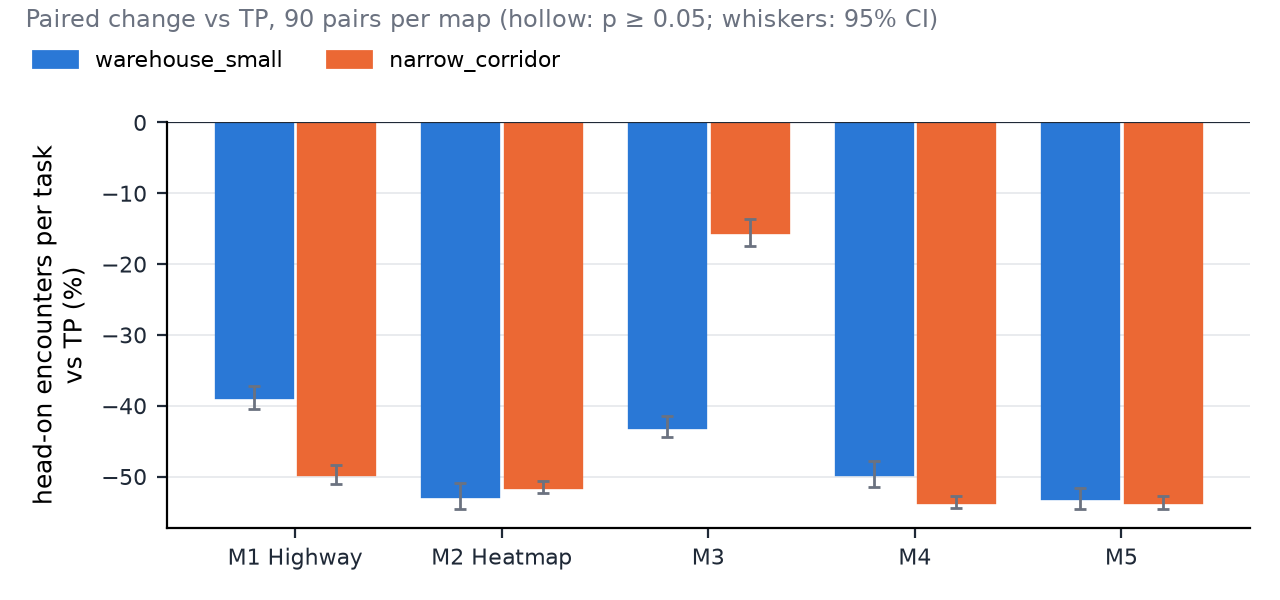
\includegraphics[width=\linewidth]{../results/summary/final_head_on.png}
  \caption{Head-on encounters per task, paired change vs.\ TP.}
  \label{fig:headon}
\end{figure}

\paragraph{Fewer encounters do not mean faster delivery; robots wait instead.}
Path costs change the mean service time by at most 2\%. On
\texttt{warehouse\_small} M2--M5 are slightly but significantly faster than TP
($-0.9\%$ to $-1.9\%$) and also lower the 95th percentile ($-0.5\%$ to
$-1.5\%$); on \texttt{narrow\_corridor} none of them differs significantly from
TP, and Highway is no faster on \texttt{warehouse\_small} and slower on
\texttt{narrow\_corridor} ($+1.1\%$). The wait fraction rises instead: by
13.5--57\% on \texttt{warehouse\_small} and by 101--145\% on
\texttt{narrow\_corridor} for every method except M3. Agents trade a head-on
encounter for waiting before an aisle, which leaves the service time almost
unchanged.

\paragraph{Contribution 1: timing matters for encounters, not for service time.}
With tuned parameters, M4 removes more encounters than M3 on both maps
($-49.7\%$ vs.\ $-43.0\%$ on \texttt{warehouse\_small}; $-53.6\%$ vs.\
$-15.5\%$ on \texttt{narrow\_corridor}). Tuning chose different window sizes
for M3 and M4 on \texttt{narrow\_corridor} (2 vs.\ $\delta=2$, i.e.\ 5 steps),
so the matched-window comparison in Section~\ref{sec:sensitivity} isolates the
effect of timing. The two do not differ in service time.

\paragraph{Contribution 2: no measurable effect of the direction term.}
M5 is within a few points of M4 on every metric (head-on $-53.1\%$ vs.\
$-49.7\%$ on \texttt{warehouse\_small}, $-53.7\%$ vs.\ $-53.6\%$ on
\texttt{narrow\_corridor}), consistent with the lane study
(Section~\ref{sec:lanes}), in which no one-way lanes form.

\paragraph{Looking forward does not beat looking backward.}
Compared directly with the tuned history heatmap M2 on the same pairs, M4 and
M5 are slightly slower on \texttt{warehouse\_small} ($+1.0\%$ and $+0.9\%$
mean service time, both significant) and indistinguishable on
\texttt{narrow\_corridor} ($+0.4\%$, not significant), where they have 4\%
fewer head-on encounters than M2 but wait 3\% more. Under heavier load (80
agents at 1 and 5 tasks per step, 20 pairs per map) M4 and M5 do lower the mean
and 95th-percentile service time on \texttt{narrow\_corridor} ($-2.5\%$ and
$-3.2\%$ for M4), but M2 does as well ($-3.0\%$ and $-3.4\%$). The forecast in
the token is exact, yet in these warehouses recent history predicts congestion
about as well.

\paragraph{Assignment helps more than routing.}
Choosing tasks with $S_{ij}$ instead of the nearest pickup lowers the mean
service time by 3.6\% on \texttt{warehouse\_small} and 1.5\% on
\texttt{narrow\_corridor} (both significant), more than any path cost
(Fig.~\ref{fig:ablation}). The gain adds to that of the path costs: M4~$+\,S_{ij}$
is 3.8\% and 1.3\% faster than TP, and adding $S_{ij}$ to M3, M4 or M5 lowers
the service time by a further 2.5--2.9\% and 1.0--1.3\%. $S_{ij}$ hardly
changes head-on encounters ($-2$\% to $-3.5\%$) and does not lengthen the
slowest tasks: on the test seeds the maximum service time is unchanged on
\texttt{warehouse\_small} ($+0.5\%$, not significant) and lower on
\texttt{narrow\_corridor} ($-1.6\%$). Routing and assignment therefore act on
different things: the path costs on encounters, the assignment on service
time.

\begin{figure}[t]
  \centering
  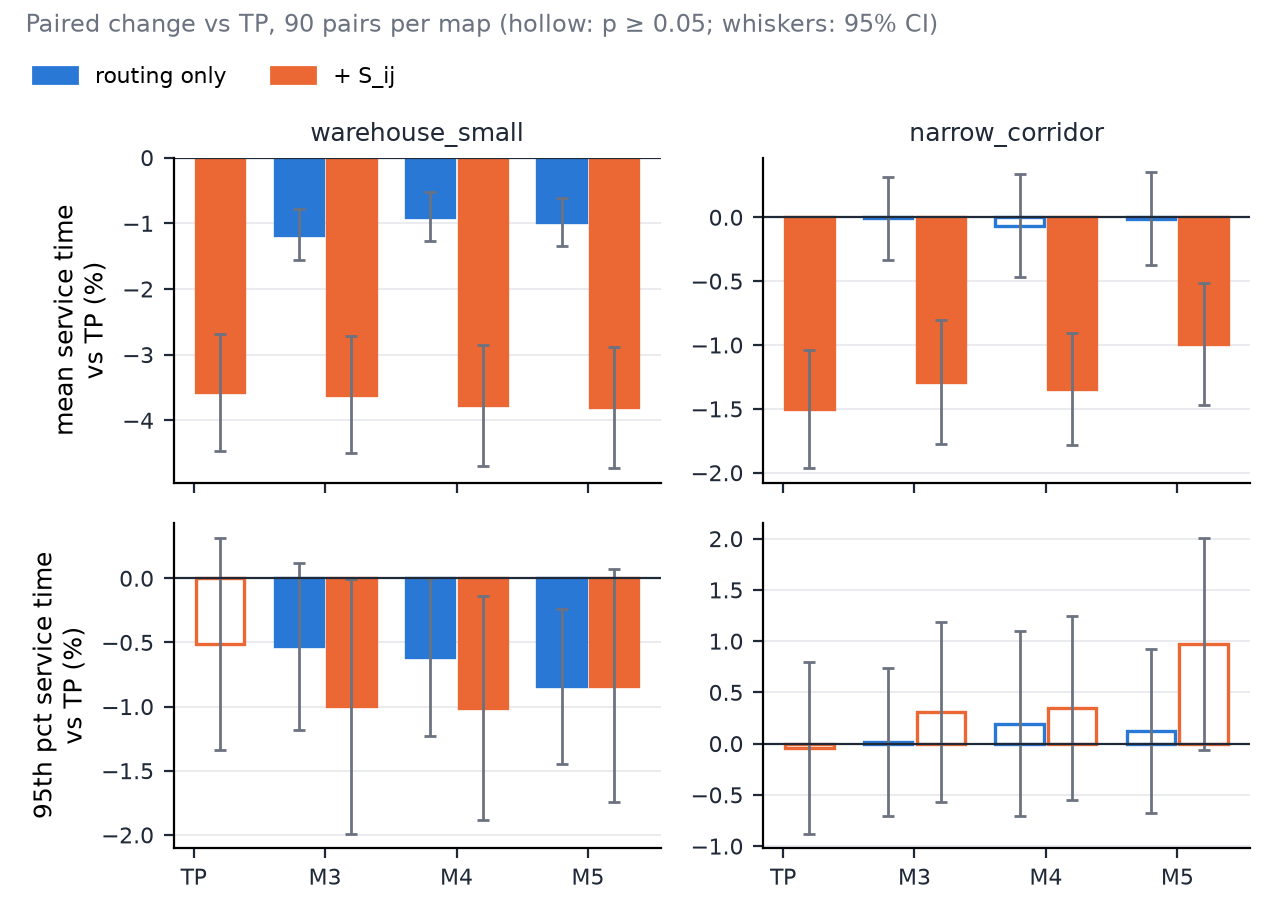
\includegraphics[width=\linewidth]{../results/summary/final_ablation.png}
  \caption{Routing vs.\ assignment: mean (top) and 95th-percentile (bottom)
  service time, paired change vs.\ TP.}
  \label{fig:ablation}
\end{figure}

\paragraph{Cost.}
Planning stays cheap. TP plans in about 0.65 ms per timestep on average on both
maps, and 1.9--2.6 ms at 80 agents. The congestion costs add 18--195\% depending on
method and map, and $S_{ij}$ adds up to 91\% on \texttt{warehouse\_small},
The slowest setting (M4, \texttt{narrow\_corridor}, 80 agents, 5 tasks per
step) averages 7.4 ms per timestep.
 from the main report. Every number below comes from
% results/summary/final.md (python experiments/final_figures.py); the table and
% figures are generated files, so rerun that script rather than editing them.
% TODO(Sicheng): \label{sec:sensitivity} and \label{sec:lanes} are referenced
% below for the matched-window and lane studies; adjust if your labels differ.

\section{Results}
\label{sec:results}

All 2{,}040 test runs completed every task with no conflicts. Table~\ref{tab:main}
gives the mean paired change of each method against TP over the 90 pairs per
map (10, 30 and 50 agents; 0.2, 1 and 5 tasks per step; seeds 0--9).
Under TP the mean service time is 122.6 timesteps on \texttt{warehouse\_small}
and 184.3 on \texttt{narrow\_corridor}, with 0.49 and 0.82 head-on encounters
per task.

\begin{table}[t]
  \centering\small
  \caption{Mean paired change vs.\ TP (\%), 90 pairs per map
  (W = \texttt{warehouse\_small}, N = \texttt{narrow\_corridor}). $^*$: Wilcoxon
  signed-rank $p<0.05$. Lower is better in every column.}
  \label{tab:main}
  % Generated by experiments/final_figures.py -- do not edit by hand.
\begin{tabular}{lrrrrrrrr}
\toprule
 & \multicolumn{2}{c}{Service time} & \multicolumn{2}{c}{p95 service} & \multicolumn{2}{c}{Head-on / task} & \multicolumn{2}{c}{Wait fraction} \\
 & W & N & W & N & W & N & W & N \\
\midrule
M1 Highway & +0.4 & +1.1$^*$ & +1.2 & +1.9$^*$ & $-$38.8$^*$ & $-$49.7$^*$ & +13.5$^*$ & +101.4$^*$ \\
M2 Heatmap & $-$1.9$^*$ & $-$0.4 & $-$1.5$^*$ & +0.1 & $-$52.8$^*$ & $-$51.5$^*$ & +22.1$^*$ & +137.8$^*$ \\
M3 & $-$1.2$^*$ & $-$0.0 & $-$0.5$^*$ & +0.0 & $-$43.0$^*$ & $-$15.5$^*$ & +17.3$^*$ & +40.8$^*$ \\
M4 & $-$0.9$^*$ & $-$0.1 & $-$0.6$^*$ & +0.2 & $-$49.7$^*$ & $-$53.6$^*$ & +56.7$^*$ & +144.8$^*$ \\
M5 & $-$1.0$^*$ & $-$0.0 & $-$0.8$^*$ & +0.1 & $-$53.1$^*$ & $-$53.7$^*$ & +44.0$^*$ & +142.6$^*$ \\
\midrule
TP + $S_{ij}$ & $-$3.6$^*$ & $-$1.5$^*$ & $-$0.5 & $-$0.0 & $-$3.5$^*$ & $-$2.0$^*$ & $-$3.5$^*$ & $-$1.9$^*$ \\
M3 + $S_{ij}$ & $-$3.6$^*$ & $-$1.3$^*$ & $-$1.0$^*$ & +0.3 & $-$42.9$^*$ & $-$18.2$^*$ & +14.5$^*$ & +32.6$^*$ \\
M4 + $S_{ij}$ & $-$3.8$^*$ & $-$1.3$^*$ & $-$1.0$^*$ & +0.3 & $-$50.7$^*$ & $-$55.0$^*$ & +51.1$^*$ & +136.5$^*$ \\
M5 + $S_{ij}$ & $-$3.8$^*$ & $-$1.0$^*$ & $-$0.8$^*$ & +1.0 & $-$53.9$^*$ & $-$55.2$^*$ & +39.2$^*$ & +136.6$^*$ \\
\bottomrule
\end{tabular}

\end{table}

\paragraph{Every congestion cost removes about half of the head-on encounters.}
Every path cost lowers head-on encounters in all 90 of 90 pairs on both maps
(Fig.~\ref{fig:headon}): by 39--53\% on \texttt{warehouse\_small} and by
50--54\% on \texttt{narrow\_corridor}, except M3 there ($-15.5\%$). The tuned
time-resolved costs M4 and M5 are among the largest reductions on both maps.

\begin{figure}[t]
  \centering
  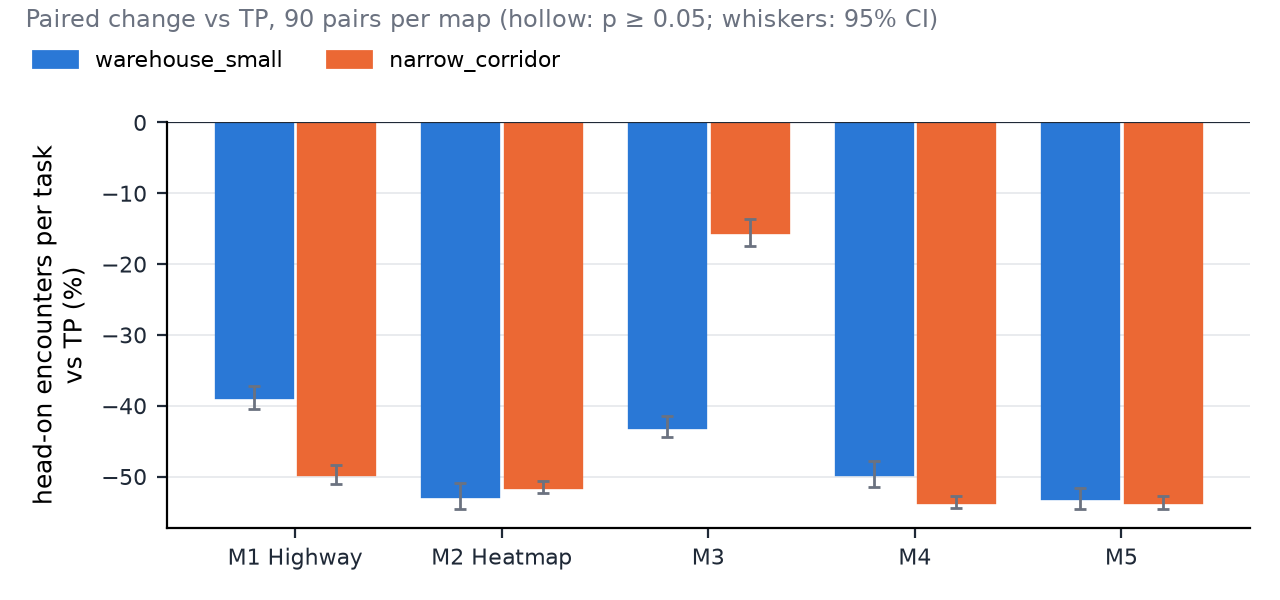
\includegraphics[width=\linewidth]{../results/summary/final_head_on.png}
  \caption{Head-on encounters per task, paired change vs.\ TP.}
  \label{fig:headon}
\end{figure}

\paragraph{Fewer encounters do not mean faster delivery; robots wait instead.}
Path costs change the mean service time by at most 2\%. On
\texttt{warehouse\_small} M2--M5 are slightly but significantly faster than TP
($-0.9\%$ to $-1.9\%$) and also lower the 95th percentile ($-0.5\%$ to
$-1.5\%$); on \texttt{narrow\_corridor} none of them differs significantly from
TP, and Highway is no faster on \texttt{warehouse\_small} and slower on
\texttt{narrow\_corridor} ($+1.1\%$). The wait fraction rises instead: by
13.5--57\% on \texttt{warehouse\_small} and by 101--145\% on
\texttt{narrow\_corridor} for every method except M3. Agents trade a head-on
encounter for waiting before an aisle, which leaves the service time almost
unchanged.

\paragraph{Contribution 1: timing matters for encounters, not for service time.}
With tuned parameters, M4 removes more encounters than M3 on both maps
($-49.7\%$ vs.\ $-43.0\%$ on \texttt{warehouse\_small}; $-53.6\%$ vs.\
$-15.5\%$ on \texttt{narrow\_corridor}). Tuning chose different window sizes
for M3 and M4 on \texttt{narrow\_corridor} (2 vs.\ $\delta=2$, i.e.\ 5 steps),
so the matched-window comparison in Section~\ref{sec:sensitivity} isolates the
effect of timing. The two do not differ in service time.

\paragraph{Contribution 2: no measurable effect of the direction term.}
M5 is within a few points of M4 on every metric (head-on $-53.1\%$ vs.\
$-49.7\%$ on \texttt{warehouse\_small}, $-53.7\%$ vs.\ $-53.6\%$ on
\texttt{narrow\_corridor}), consistent with the lane study
(Section~\ref{sec:lanes}), in which no one-way lanes form.

\paragraph{Looking forward does not beat looking backward.}
Compared directly with the tuned history heatmap M2 on the same pairs, M4 and
M5 are slightly slower on \texttt{warehouse\_small} ($+1.0\%$ and $+0.9\%$
mean service time, both significant) and indistinguishable on
\texttt{narrow\_corridor} ($+0.4\%$, not significant), where they have 4\%
fewer head-on encounters than M2 but wait 3\% more. Under heavier load (80
agents at 1 and 5 tasks per step, 20 pairs per map) M4 and M5 do lower the mean
and 95th-percentile service time on \texttt{narrow\_corridor} ($-2.5\%$ and
$-3.2\%$ for M4), but M2 does as well ($-3.0\%$ and $-3.4\%$). The forecast in
the token is exact, yet in these warehouses recent history predicts congestion
about as well.

\paragraph{Assignment helps more than routing.}
Choosing tasks with $S_{ij}$ instead of the nearest pickup lowers the mean
service time by 3.6\% on \texttt{warehouse\_small} and 1.5\% on
\texttt{narrow\_corridor} (both significant), more than any path cost
(Fig.~\ref{fig:ablation}). The gain adds to that of the path costs: M4~$+\,S_{ij}$
is 3.8\% and 1.3\% faster than TP, and adding $S_{ij}$ to M3, M4 or M5 lowers
the service time by a further 2.5--2.9\% and 1.0--1.3\%. $S_{ij}$ hardly
changes head-on encounters ($-2$\% to $-3.5\%$) and does not lengthen the
slowest tasks: on the test seeds the maximum service time is unchanged on
\texttt{warehouse\_small} ($+0.5\%$, not significant) and lower on
\texttt{narrow\_corridor} ($-1.6\%$). Routing and assignment therefore act on
different things: the path costs on encounters, the assignment on service
time.

\begin{figure}[t]
  \centering
  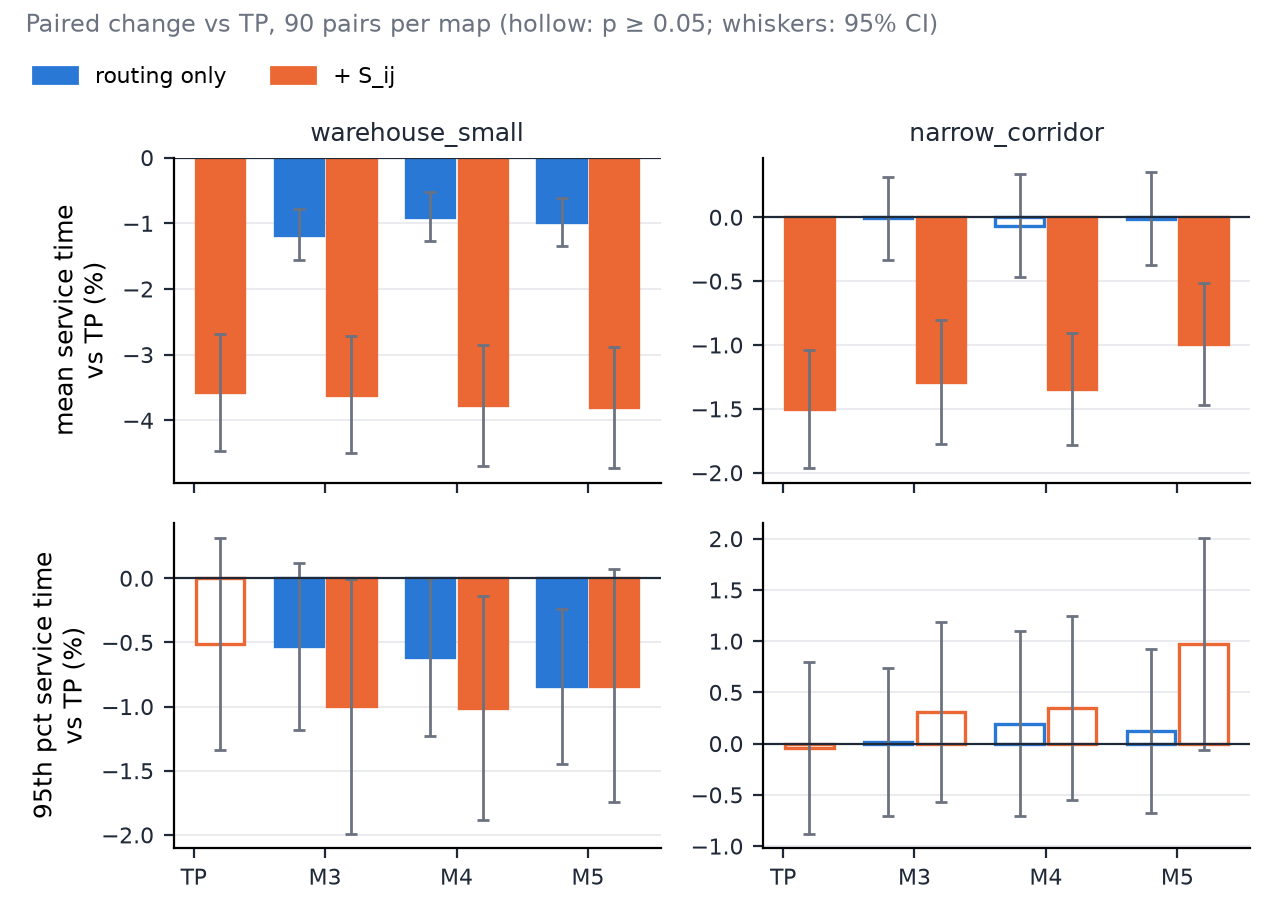
\includegraphics[width=\linewidth]{../results/summary/final_ablation.png}
  \caption{Routing vs.\ assignment: mean (top) and 95th-percentile (bottom)
  service time, paired change vs.\ TP.}
  \label{fig:ablation}
\end{figure}

\paragraph{Cost.}
Planning stays cheap. TP plans in about 0.65 ms per timestep on average on both
maps, and 1.9--2.6 ms at 80 agents. The congestion costs add 18--195\% depending on
method and map, and $S_{ij}$ adds up to 91\% on \texttt{warehouse\_small},
The slowest setting (M4, \texttt{narrow\_corridor}, 80 agents, 5 tasks per
step) averages 7.4 ms per timestep.
 from the main report. Every number below comes from
% results/summary/final.md (python experiments/final_figures.py); the table and
% figures are generated files, so rerun that script rather than editing them.
% TODO(Sicheng): \label{sec:sensitivity} and \label{sec:lanes} are referenced
% below for the matched-window and lane studies; adjust if your labels differ.

\section{Results}
\label{sec:results}

All 2{,}040 test runs completed every task with no conflicts. Table~\ref{tab:main}
gives the mean paired change of each method against TP over the 90 pairs per
map (10, 30 and 50 agents; 0.2, 1 and 5 tasks per step; seeds 0--9).
Under TP the mean service time is 122.6 timesteps on \texttt{warehouse\_small}
and 184.3 on \texttt{narrow\_corridor}, with 0.49 and 0.82 head-on encounters
per task.

\begin{table}[t]
  \centering\small
  \caption{Mean paired change vs.\ TP (\%), 90 pairs per map
  (W = \texttt{warehouse\_small}, N = \texttt{narrow\_corridor}). $^*$: Wilcoxon
  signed-rank $p<0.05$. Lower is better in every column.}
  \label{tab:main}
  % Generated by experiments/final_figures.py -- do not edit by hand.
\begin{tabular}{lrrrrrrrr}
\toprule
 & \multicolumn{2}{c}{Service time} & \multicolumn{2}{c}{p95 service} & \multicolumn{2}{c}{Head-on / task} & \multicolumn{2}{c}{Wait fraction} \\
 & W & N & W & N & W & N & W & N \\
\midrule
M1 Highway & +0.4 & +1.1$^*$ & +1.2 & +1.9$^*$ & $-$38.8$^*$ & $-$49.7$^*$ & +13.5$^*$ & +101.4$^*$ \\
M2 Heatmap & $-$1.9$^*$ & $-$0.4 & $-$1.5$^*$ & +0.1 & $-$52.8$^*$ & $-$51.5$^*$ & +22.1$^*$ & +137.8$^*$ \\
M3 & $-$1.2$^*$ & $-$0.0 & $-$0.5$^*$ & +0.0 & $-$43.0$^*$ & $-$15.5$^*$ & +17.3$^*$ & +40.8$^*$ \\
M4 & $-$0.9$^*$ & $-$0.1 & $-$0.6$^*$ & +0.2 & $-$49.7$^*$ & $-$53.6$^*$ & +56.7$^*$ & +144.8$^*$ \\
M5 & $-$1.0$^*$ & $-$0.0 & $-$0.8$^*$ & +0.1 & $-$53.1$^*$ & $-$53.7$^*$ & +44.0$^*$ & +142.6$^*$ \\
\midrule
TP + $S_{ij}$ & $-$3.6$^*$ & $-$1.5$^*$ & $-$0.5 & $-$0.0 & $-$3.5$^*$ & $-$2.0$^*$ & $-$3.5$^*$ & $-$1.9$^*$ \\
M3 + $S_{ij}$ & $-$3.6$^*$ & $-$1.3$^*$ & $-$1.0$^*$ & +0.3 & $-$42.9$^*$ & $-$18.2$^*$ & +14.5$^*$ & +32.6$^*$ \\
M4 + $S_{ij}$ & $-$3.8$^*$ & $-$1.3$^*$ & $-$1.0$^*$ & +0.3 & $-$50.7$^*$ & $-$55.0$^*$ & +51.1$^*$ & +136.5$^*$ \\
M5 + $S_{ij}$ & $-$3.8$^*$ & $-$1.0$^*$ & $-$0.8$^*$ & +1.0 & $-$53.9$^*$ & $-$55.2$^*$ & +39.2$^*$ & +136.6$^*$ \\
\bottomrule
\end{tabular}

\end{table}

\paragraph{Every congestion cost removes about half of the head-on encounters.}
Every path cost lowers head-on encounters in all 90 of 90 pairs on both maps
(Fig.~\ref{fig:headon}): by 39--53\% on \texttt{warehouse\_small} and by
50--54\% on \texttt{narrow\_corridor}, except M3 there ($-15.5\%$). The tuned
time-resolved costs M4 and M5 are among the largest reductions on both maps.

\begin{figure}[t]
  \centering
  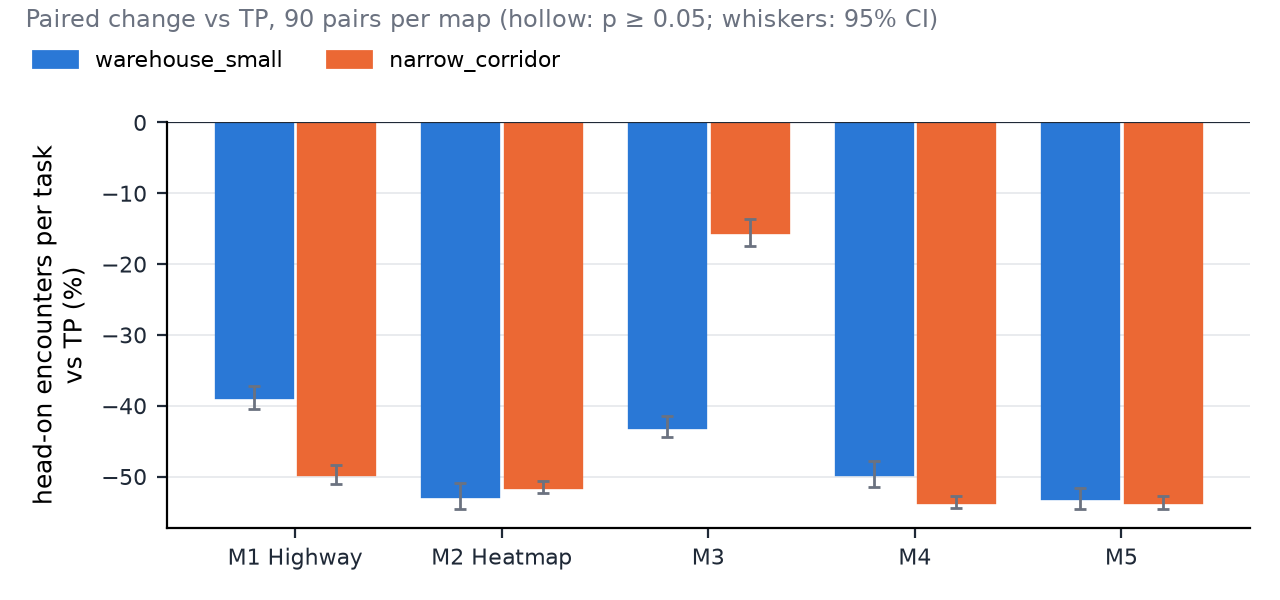
\includegraphics[width=\linewidth]{../results/summary/final_head_on.png}
  \caption{Head-on encounters per task, paired change vs.\ TP.}
  \label{fig:headon}
\end{figure}

\paragraph{Fewer encounters do not mean faster delivery; robots wait instead.}
Path costs change the mean service time by at most 2\%. On
\texttt{warehouse\_small} M2--M5 are slightly but significantly faster than TP
($-0.9\%$ to $-1.9\%$) and also lower the 95th percentile ($-0.5\%$ to
$-1.5\%$); on \texttt{narrow\_corridor} none of them differs significantly from
TP, and Highway is no faster on \texttt{warehouse\_small} and slower on
\texttt{narrow\_corridor} ($+1.1\%$). The wait fraction rises instead: by
13.5--57\% on \texttt{warehouse\_small} and by 101--145\% on
\texttt{narrow\_corridor} for every method except M3. Agents trade a head-on
encounter for waiting before an aisle, which leaves the service time almost
unchanged.

\paragraph{Contribution 1: timing matters for encounters, not for service time.}
With tuned parameters, M4 removes more encounters than M3 on both maps
($-49.7\%$ vs.\ $-43.0\%$ on \texttt{warehouse\_small}; $-53.6\%$ vs.\
$-15.5\%$ on \texttt{narrow\_corridor}). Tuning chose different window sizes
for M3 and M4 on \texttt{narrow\_corridor} (2 vs.\ $\delta=2$, i.e.\ 5 steps),
so the matched-window comparison in Section~\ref{sec:sensitivity} isolates the
effect of timing. The two do not differ in service time.

\paragraph{Contribution 2: no measurable effect of the direction term.}
M5 is within a few points of M4 on every metric (head-on $-53.1\%$ vs.\
$-49.7\%$ on \texttt{warehouse\_small}, $-53.7\%$ vs.\ $-53.6\%$ on
\texttt{narrow\_corridor}), consistent with the lane study
(Section~\ref{sec:lanes}), in which no one-way lanes form.

\paragraph{Looking forward does not beat looking backward.}
Compared directly with the tuned history heatmap M2 on the same pairs, M4 and
M5 are slightly slower on \texttt{warehouse\_small} ($+1.0\%$ and $+0.9\%$
mean service time, both significant) and indistinguishable on
\texttt{narrow\_corridor} ($+0.4\%$, not significant), where they have 4\%
fewer head-on encounters than M2 but wait 3\% more. Under heavier load (80
agents at 1 and 5 tasks per step, 20 pairs per map) M4 and M5 do lower the mean
and 95th-percentile service time on \texttt{narrow\_corridor} ($-2.5\%$ and
$-3.2\%$ for M4), but M2 does as well ($-3.0\%$ and $-3.4\%$). The forecast in
the token is exact, yet in these warehouses recent history predicts congestion
about as well.

\paragraph{Assignment helps more than routing.}
Choosing tasks with $S_{ij}$ instead of the nearest pickup lowers the mean
service time by 3.6\% on \texttt{warehouse\_small} and 1.5\% on
\texttt{narrow\_corridor} (both significant), more than any path cost
(Fig.~\ref{fig:ablation}). The gain adds to that of the path costs: M4~$+\,S_{ij}$
is 3.8\% and 1.3\% faster than TP, and adding $S_{ij}$ to M3, M4 or M5 lowers
the service time by a further 2.5--2.9\% and 1.0--1.3\%. $S_{ij}$ hardly
changes head-on encounters ($-2$\% to $-3.5\%$) and does not lengthen the
slowest tasks: on the test seeds the maximum service time is unchanged on
\texttt{warehouse\_small} ($+0.5\%$, not significant) and lower on
\texttt{narrow\_corridor} ($-1.6\%$). Routing and assignment therefore act on
different things: the path costs on encounters, the assignment on service
time.

\begin{figure}[t]
  \centering
  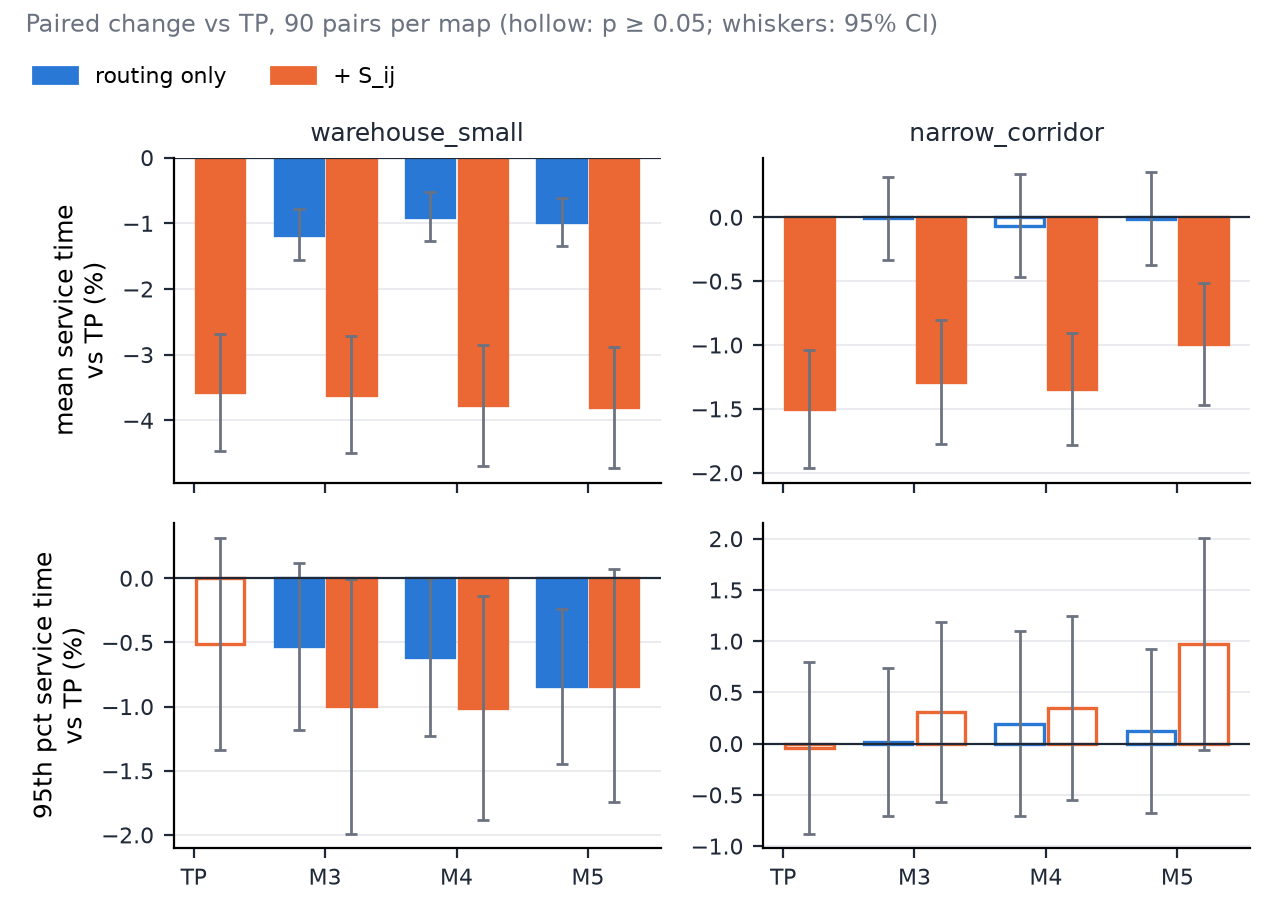
\includegraphics[width=\linewidth]{../results/summary/final_ablation.png}
  \caption{Routing vs.\ assignment: mean (top) and 95th-percentile (bottom)
  service time, paired change vs.\ TP.}
  \label{fig:ablation}
\end{figure}

\paragraph{Cost.}
Planning stays cheap. TP plans in about 0.65 ms per timestep on average on both
maps, and 1.9--2.6 ms at 80 agents. The congestion costs add 18--195\% depending on
method and map, and $S_{ij}$ adds up to 91\% on \texttt{warehouse\_small},
The slowest setting (M4, \texttt{narrow\_corridor}, 80 agents, 5 tasks per
step) averages 7.4 ms per timestep.
